\documentclass[10pt,journal,a4paper]{IEEEtran}
% \includegraphics
\usepackage{amsmath,amssymb,mathrsfs}
\usepackage{bm}
\usepackage{graphicx}
\usepackage{caption}
\usepackage{subcaption}
\usepackage{url}

\usepackage[ruled,vlined]{algorithm2e}


\newtheorem{lemma}{Lemma}
\newtheorem{theorem}{Theorem}
%\newtheorem{proposition}[lemma]{Proposition}
\newtheorem{corollary}{Corollary}
\newtheorem{definition}{Definition}
\newtheorem{remark}{Remark}
%\newtheorem{claim}[theorem]{Claim}
%\newtheorem{fact}[lemma]{Fact}
%\newtheorem{example}[lemma]{Example}
%\newtheorem{exercise}{Exercise}
\newtheorem{assumption}{Assumption}

\newcommand\myp{\pause}
% \newcommand\myp{}


\newcommand{\aaaa}{\mathrm{(a)}}
\newcommand{\bbbb}{\mathrm{(b)}}
\newcommand{\cccc}{\mathrm{(c)}}
\newcommand{\dddd}{\mathrm{(d)}}
\newcommand{\eeee}{\mathrm{(e)}}
\newcommand{\ffff}{\mathrm{(f)}}
\newcommand{\gggg}{\mathrm{(g)}}
\newcommand{\hhhh}{\mathrm{(h)}}
\newcommand{\iiii}{\mathrm{(i)}}
\newcommand{\jjjj}{\mathrm{(j)}}
\newcommand{\kkkk}{\mathrm{(k)}}
\newcommand{\llll}{\mathrm{(l)}}
\newcommand{\mmmm}{\mathrm{(m)}}
\newcommand{\nnnn}{\mathrm{(n)}}
\newcommand{\oooo}{\mathrm{(o)}}
\newcommand{\pppp}{\mathrm{(p)}}
\newcommand{\qqqq}{\mathrm{(q)}}
\newcommand{\rrrr}{\mathrm{(r)}}
\newcommand{\ssss}{\mathrm{(s)}}
\newcommand{\tttt}{\mathrm{(t)}}

\newcommand{\lp}{\left(}
\newcommand{\rp}{\right)}
\newcommand{\lb}{\left[}
\newcommand{\rb}{\right]}
\newcommand{\mv}{\middle\vert}
\newcommand{\lv}{\left\vert}
\newcommand{\rv}{\right\vert}
\newcommand{\lV}{\left\Vert}
\newcommand{\rV}{\right\Vert}
\newcommand{\lbp}{\left\{}
\newcommand{\rbp}{\right\}}
\newcommand{\ul}{\underline}
\newcommand{\ol}{\overline}
\newcommand{\mcal}{\mathcal}
\newcommand{\mscr}{\mathscr}
\newcommand{\mrm}{\mathrm}
\newcommand{\what}{\widehat}
\newcommand{\wtild}{\widetilde}
\newcommand{\mb}{\mathbf}
\newcommand{\mbb}{\mathbb}
\newcommand{\msf}{\mathsf}
\newcommand{\la}{\leftarrow}
\newcommand{\ra}{\rightarrow}
\newcommand{\Ra}{\Rightarrow}
\newcommand{\La}{\Leftarrow}

\newcommand{\lang}{\left\langle}
\newcommand{\rang}{\right\rangle}

\newcommand{\etal}{{\it et al.}}

\newcommand{\indi}[1]{\mathds{1} \lbp #1 \rbp}

\DeclareMathOperator*{\argmax}{arg\,max}
\DeclareMathOperator*{\argmin}{arg\,min}
\DeclareMathOperator*{\argsup}{arg\,sup}
\DeclareMathOperator*{\arginf}{arg\,inf}
\DeclareMathOperator{\Tr}{Tr}
\DeclareMathOperator*{\expt}{\mbb{E}}
\DeclareMathOperator{\diag}{\textbf{diag}}
\DeclareMathOperator{\cov}{Cov}
\DeclareMathOperator{\range}{range}
\DeclareMathOperator{\poly}{\text{poly}}
\DeclareMathOperator{\nan}{\texttt{NaN}}
\DeclareMathOperator{\prob}{\mathbb{P}}


\newcounter{MYtempeqncnt}

\allowdisplaybreaks


\usepackage{balance}
\begin{document}
%
% paper title
% can use linebreaks \\ within to get better formatting as desired
\title{Generating Occlusion-free Vehicle Images From Occluded Vehicle Images Based on the Drone Dataset}
%
% 
\author{Student: Yifeng Chen, Supervisor: Yura Tak, Robert Fonod, Professor: Nikolas Geroliminis 


\textit{\'Ecole Polytechnique F\'ed\'erale de Lausanne, Switzerland}}

\IEEEcompsoctitleabstractindextext{
\begin{abstract}
Occluded vehicles, as a common phenomenon in the drone dataset, have a negative impact on traffic monitoring in Unmanned Aerial Systems. Due to the lack of occluded-free and occluded pair vehicle datasets, few researchers focus on solving the vehicle occlusion removal problem. Nevertheless, several types of research focus on solving the occluded faces problems and achieving significant results. To this end, we build our own occluded vehicle dataset on this project. Besides, inspired by the occluded faces removing problem, we propose an updated context encoder – a convolutional neural network trained to generate the contents of an arbitrary image region conditioned on its surroundings.  Compared to the original context encoder, which could reconstruct the image based on a fixed-size binary mask in a fixed location, our updated context encoder could reconstruct the image based on a flexible fixed-size mask with a random location. Sharper results could be obtained by implementing the pixel-wise reconstruction loss and an adversarial loss. We create an occluded vehicle dataset from the Pully dataset and several occlusions. We evaluate the performance of the pre-trained context encoder on the occluded vehicle image dataset, including tree and shadow. The experimental results demonstrate that our work can effectively reconstruct the vehicle image.
\end{abstract}
}

% make the title area
\maketitle
\IEEEdisplaynotcompsoctitleabstractindextext


\section{Introduction}
To obtain a better understanding of the libraries for deep learning like Pytorch, we develop some of the modules by ourselves for the second mini-project. In this project, we will implement our own framework to denoise images without using autograd or torch.nn modules.

Instead of applying the Unet structure illustrated in mini-project 1, we implement a simple structure mentioned in the mini-project 2 description, which combines 2 convolutional layers, 3 Relu activation functions, 2 upsampling layers and 1 sigmoid activation function. Besides, mean square error loss criteria is applied and stochastic gradient descent optimizer is implemented. We train our architecture based on the train dataset(50000 samples) and test our architecture based on the validation dataset(1000 samples), and still get satisfied results, where psnr value is 22.81dB.
\section{Methods} \label{sec: methods}

\subsection{Functional traffic network construction} \label{sec: network construction}
In order to analyze the percolation transition in dynamic traffic network, a framework is built based on percolation theory \cite{li2015percolation}. Instead of constructing a network based on the structure topology, only roads in the network with a speed greater than a specified threshold are considered functionally linked in this framework. The construction process is illustrated below:

Roads in real-world traffic networks can be divided into distinct states based on their speed. A road is considered as functional only if its velocity level meets a given demand. A variable threshold $ q \in [0, 1]$ is set to denote the speed demand of drivers at a given time. Measured data of speed is sorted during a long period of time for each road segment in increasing order, the 95 percentile is chosen as the standard maximal value of this road $v_{i j}^m$. Then the speed $v_{i j}(t)$ of each road from site $i$ to site $j$ at time is normalized to get the relative speed, $r_{i j} =v_{i j}(t)/v_{i j}^m$. Since the road network is a directed graph, $v_{i j}(t)$ is usually different from $v_{j i}(t)$ due to the direction of the traffic flow. For traffic state in each road segment, a comparison is made between the relative speed 
$r_{i j}(t)$ and the given threshold $q$. If $r_{i j}(t) \geq q$, the road section is functional because it satisfies demand; otherwise, it is dysfunctional and should be removed from the original road network.



\subsection{Critical threshold $q_c$}
We construct a functional network of the traffic dynamics from the original topology for any given $q$. If $q=0$, every road section meets demand, and the functioning traffic network is identical to the previous network. On the other hand, if $q=1$, since almost all the links are removed from the original network, the functional network becomes completely fragmented. The functional traffic network becomes diluted as $q$ grows from 0 to 1, which is known as "traffic percolation". $q_c(t)$ is the crucial threshold value of $q$ in traffic percolation, where the huge component of the dynamical network breaks down into fragmented local traffic clusters and the second biggest cluster reaches its maximum size \cite{li2015percolation, zeng2019switch}.


\begin{figure*}[hbt!]
\centering
\begin{subfigure}[t]{0.3\linewidth}
    \centering
    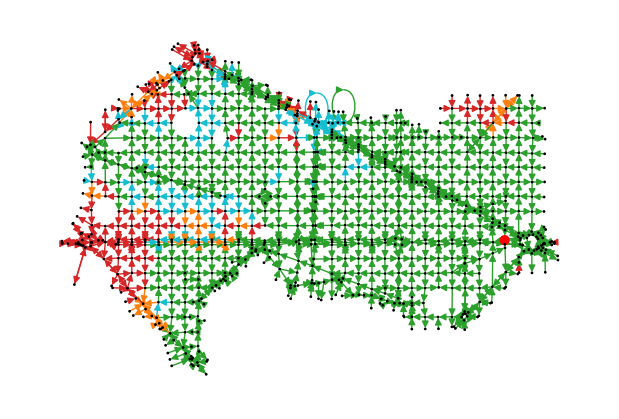
\includegraphics[width=\linewidth]{images/reachable/first_normal_1.png}
    \caption{Starting point 1, normal period}
    \label{fig: first normal reachable}
\end{subfigure}
\begin{subfigure}[t]{0.3\linewidth}
    \centering
    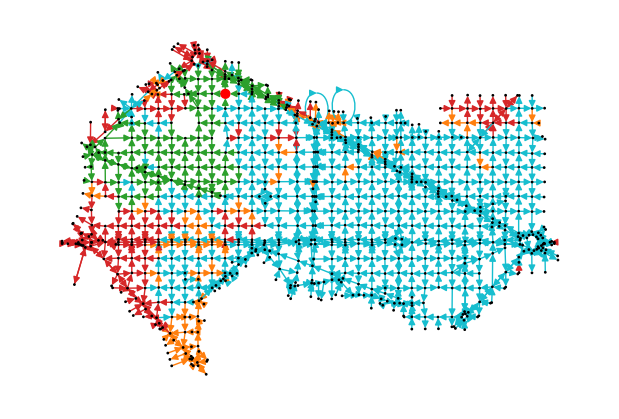
\includegraphics[width=\linewidth]{images/reachable/second_normal_1.png}
    \caption{Starting point 2, normal period}
    \label{fig: second normal reachable}
\end{subfigure}
\begin{subfigure}[t]{0.3\linewidth}
    \centering
    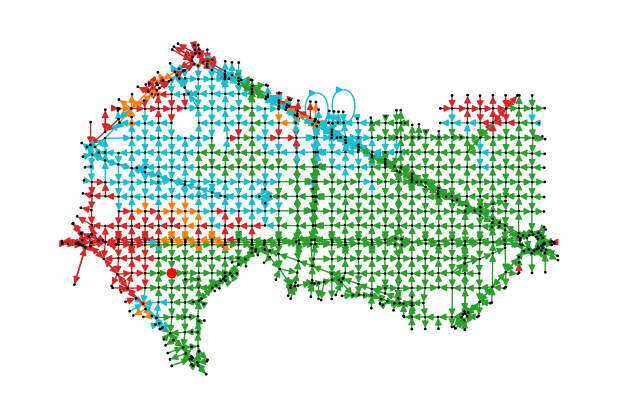
\includegraphics[width=\linewidth]{images/reachable/third_normal_1.png}
    \caption{Starting point 3, normal period}
    \label{fig: third normal reachalbe}
\end{subfigure}
\hfill
\begin{subfigure}[t]{0.3\linewidth}
    \centering
    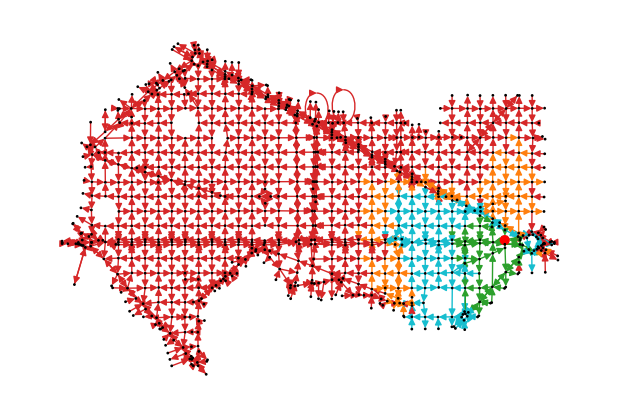
\includegraphics[width=\linewidth]{images/reachable/first_busy_1.png}
    \caption{Starting point 1, busy period}
    \label{fig: first busy reachable}
\end{subfigure}
\begin{subfigure}[t]{0.3\linewidth}
    \centering
    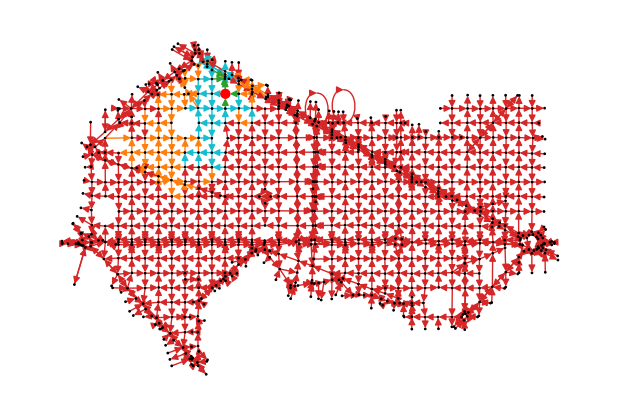
\includegraphics[width=\linewidth]{images/reachable/second_busy_1.png}
    \caption{Starting point 2, busy period}
    \label{fig: second busy reachable}
\end{subfigure}
\begin{subfigure}[t]{0.3\linewidth}
    \centering
    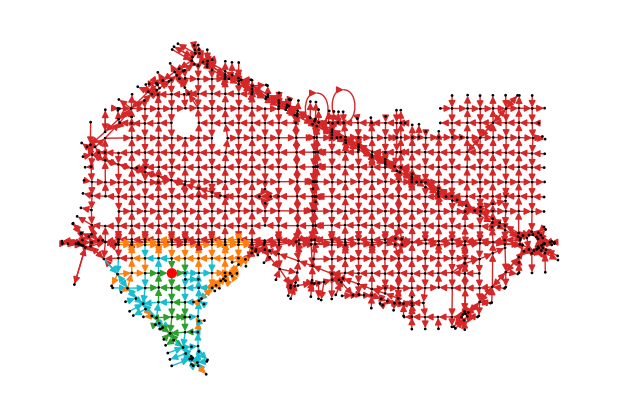
\includegraphics[width=\linewidth]{images/reachable/third_busy_1.png}
    \caption{Starting point 3, busy period}
    \label{fig: third busy reachable}
\end{subfigure}
\caption{The reachable area from different starting points (the red spot in green area). Green roads represent 1 minute reachable; blue for 2; orange for 3; and red for $>4$. We choose \textit{busy period} and \textit{normal period} mark.}
\hfill
\label{fig: reachable areas}
\end{figure*}




\subsection{Introduction of the bottleneck}
When we increase the $q$ value slightly above the crucial threshold $q_c$, several links are removed. While some links are removed accidentally, some links play an important function in linking distinct local traffic clusters in the traffic network. Only these links are considered as bottleneck roads, as their improvement will decide the critical threshold $q_c$ \cite{li2015percolation}.


\subsection{Network type and cluster power law}
City design varies in all cities. 2D grid is the most common topology, but it changes with different terrain and highway links. Specifically, the network would become more like a small-world model with more high speed links between distant locations. 

By the network constructed using the method stated in Section \ref{sec: network construction}, the connected components size and numbers follows a power rule as (\ref{eq: power law}) when we choose $q \simeq q_c$. 
\begin{equation} \label{eq: power law}
    n_s \sim s^{-\tau}
\end{equation}
where $n_s$ is the ratio between the number
of s-sized clusters and the total number of clusters; $s$ is the cluster size; and $\tau$ is the corresponding critical percolation exponent \cite{zeng2019switch}. 


The theoretical percolation exponent of a 2D grid is $\tau_{grid}^{(2)} = 2.05$, and for a small-world model is $\tau_{sw} = 2.5$ \cite{zeng2019switch, huang2018critical}. Thus, we can determine the type of network by comparing the empirical $\tau$. Since the traffic network is a spatial-temporal system \cite{zeng2019switch}, we check not only the static structure of the network, but also the evolution of $\tau$ across time. Generally, a road system is more resilient when it is able to maintain more high speed links under heavy traffic.

\section{Result} \label{sec: result}

% \begin{figure}[t]
%     \centering
%     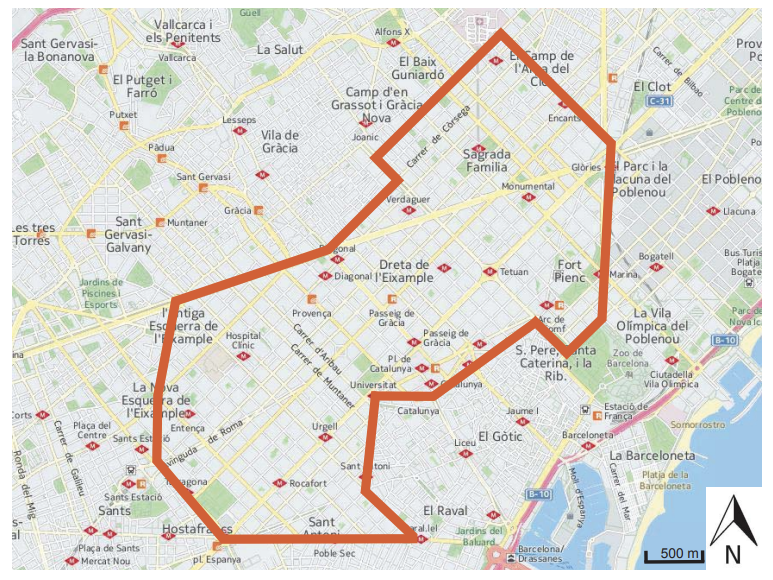
\includegraphics[width=0.9\linewidth]{images/Map of studied area.png}
%     \caption{Studied area in Barcelona, Spain. ({Source: \protect\url{http://maps.here.com}}) }
%     \label{fig: barcelona map}
% \end{figure}

\subsection{Dataset and the functional netwrok model}

\subsubsection{Dataset description}
The urban network of Barcelona, Spain is used as the test site (see Fig \ref{fig: barcelona map} for a representation of the studied area on the map). The network covers an area of 12 square kilometers with about 600 intersections and 1500 links of various lengths.

The traffic flow data is acquired based on a micro simulation experiment \cite{kouvelas2017enhancing}. The duration of this simulation is 1 hour, the speed of each link is measured for each 90 seconds. The dataset of this experiment represents an evolution of congestion in this area. At the beginning, the vehicle can pass in most area with a free flow speed. With the increasing of the time, the road network becomes congestion.

\subsubsection{Network model representation}
As stated in Section \ref{sec: network construction}, we formulate the abstract network model with a specific construction method. To verify the fidelity of the model, one can observe the reachable area within a specific time as presented in Fig \ref{fig: reachable areas}. We select 3 points from the 3 main connected components presented in Fig \ref{fig: q=0.09}, and test the reachable area during busy period and normal period. We can see that the reachable area changes a lot between both scenarios, and this division of areas conceptually represents the different connected components in the constructed network. Thus, congestion in certain roads can indeed lead to division of network in terms of traversable areas.


% \begin{figure*}[hbt!]
% \centering
% \begin{subfigure}[t]{0.3\linewidth}
%     \centering
%     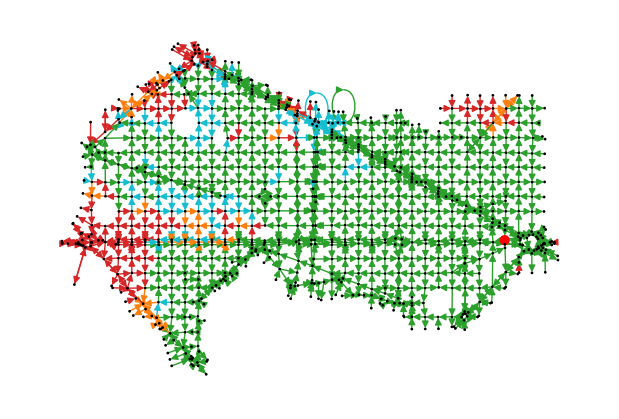
\includegraphics[width=\linewidth]{images/reachable/first_normal_1.png}
%     \caption{Starting point 1, normal period}
%     \label{fig: first normal reachable}
% \end{subfigure}
% \begin{subfigure}[t]{0.3\linewidth}
%     \centering
%     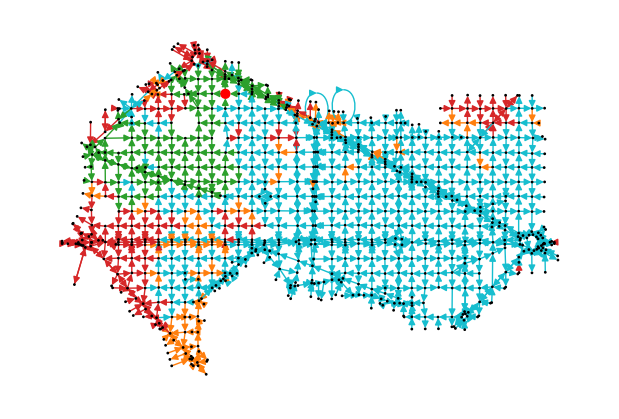
\includegraphics[width=\linewidth]{images/reachable/second_normal_1.png}
%     \caption{Starting point 2, normal period}
%     \label{fig: second normal reachable}
% \end{subfigure}
% \begin{subfigure}[t]{0.3\linewidth}
%     \centering
%     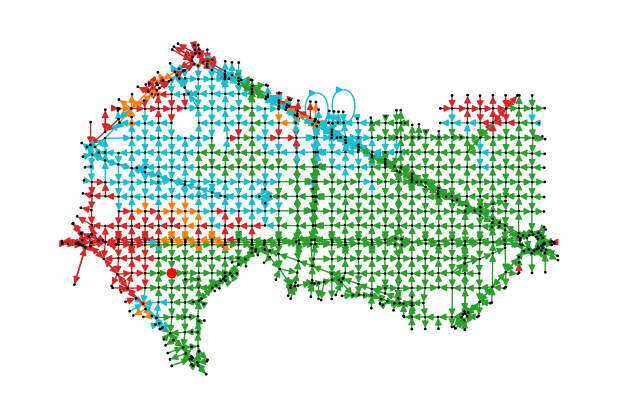
\includegraphics[width=\linewidth]{images/reachable/third_normal_1.png}
%     \caption{Starting point 3, normal period}
%     \label{fig: third normal reachalbe}
% \end{subfigure}
% \hfill
% \begin{subfigure}[t]{0.3\linewidth}
%     \centering
%     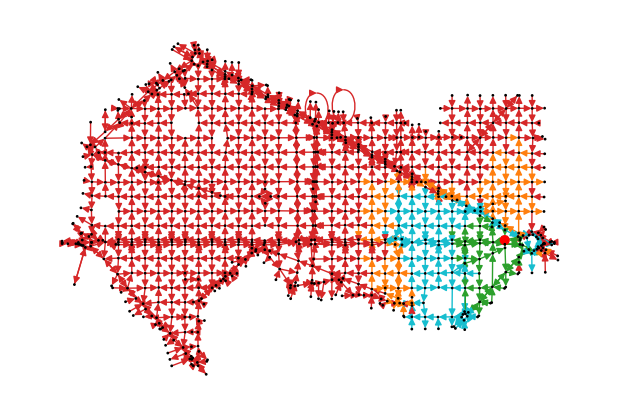
\includegraphics[width=\linewidth]{images/reachable/first_busy_1.png}
%     \caption{Starting point 1, busy period}
%     \label{fig: first busy reachable}
% \end{subfigure}
% \begin{subfigure}[t]{0.3\linewidth}
%     \centering
%     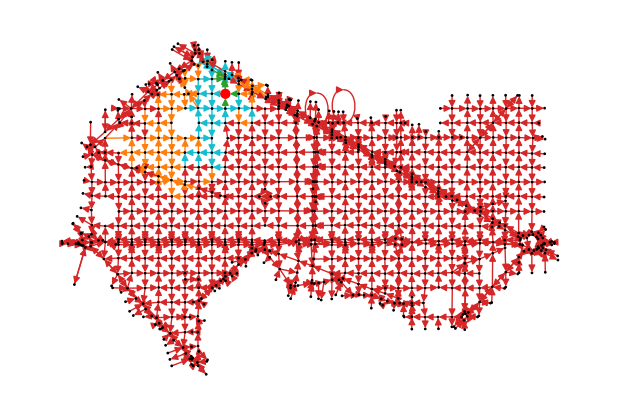
\includegraphics[width=\linewidth]{images/reachable/second_busy_1.png}
%     \caption{Starting point 2, busy period}
%     \label{fig: second busy reachable}
% \end{subfigure}
% \begin{subfigure}[t]{0.3\linewidth}
%     \centering
%     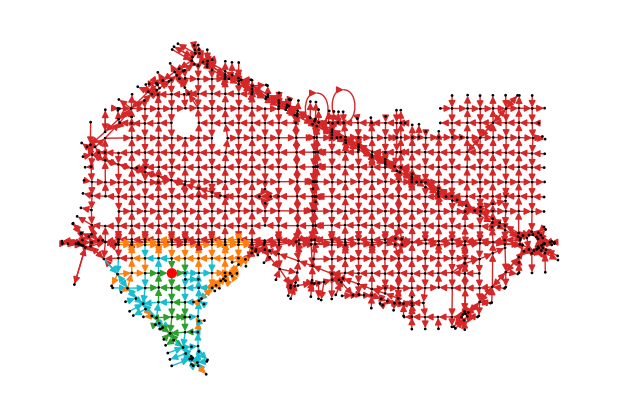
\includegraphics[width=\linewidth]{images/reachable/third_busy_1.png}
%     \caption{Starting point 3, busy period}
%     \label{fig: third busy reachable}
% \end{subfigure}
% \caption{The reachable area from different starting points (the red spot in green area). Green roads represent 1 minute reachable; blue for 2; orange for 3; and red for $>4$. We choose \textit{busy period} at 58 minute and \textit{normal period} at 117 minute mark.}
% \hfill
% \label{fig: reachable areas}
% \end{figure*}


\subsection{Analysis of percolation in road network}

\begin{figure*}[htb]
\centering
\begin{subfigure}[b]{0.25\textwidth}
    \centering
    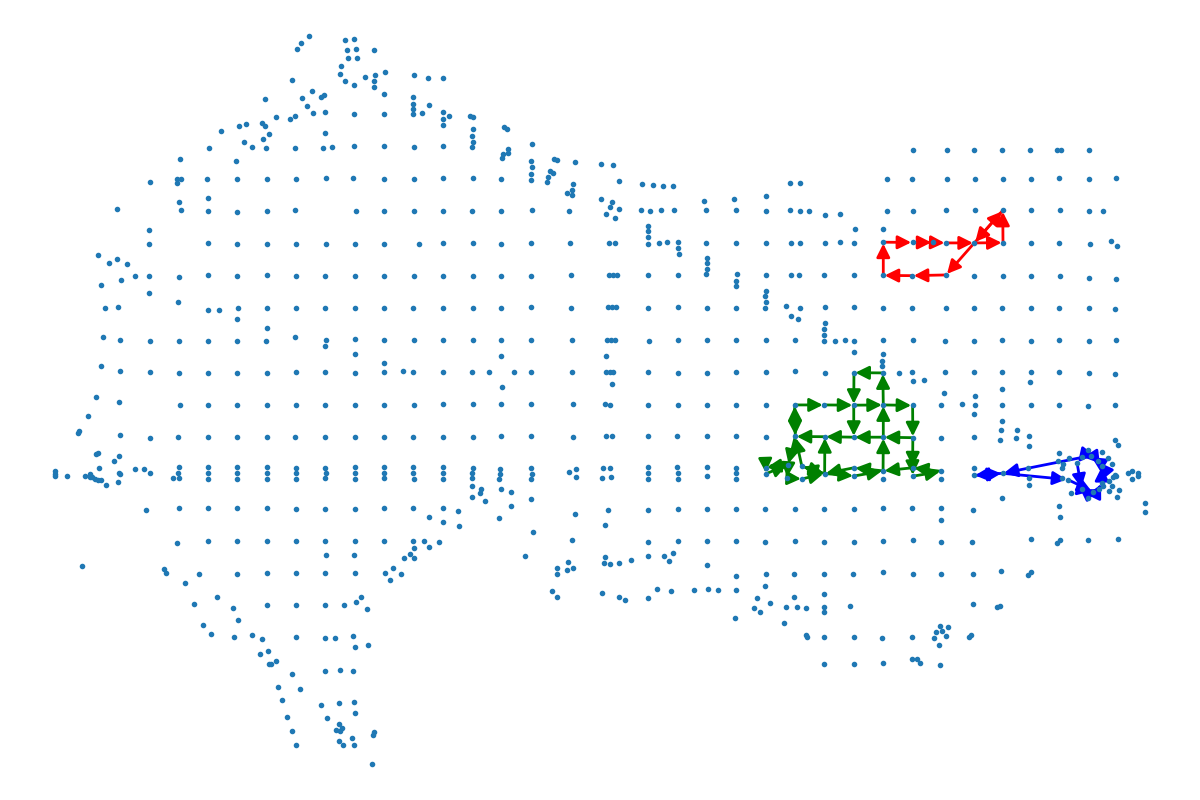
\includegraphics[width=\linewidth]{images/069.png}
    \caption{$q=0.69$}
    \label{fig: q=0.69}
\end{subfigure}
\hfill
\begin{subfigure}[b]{0.25\textwidth}
    \centering
    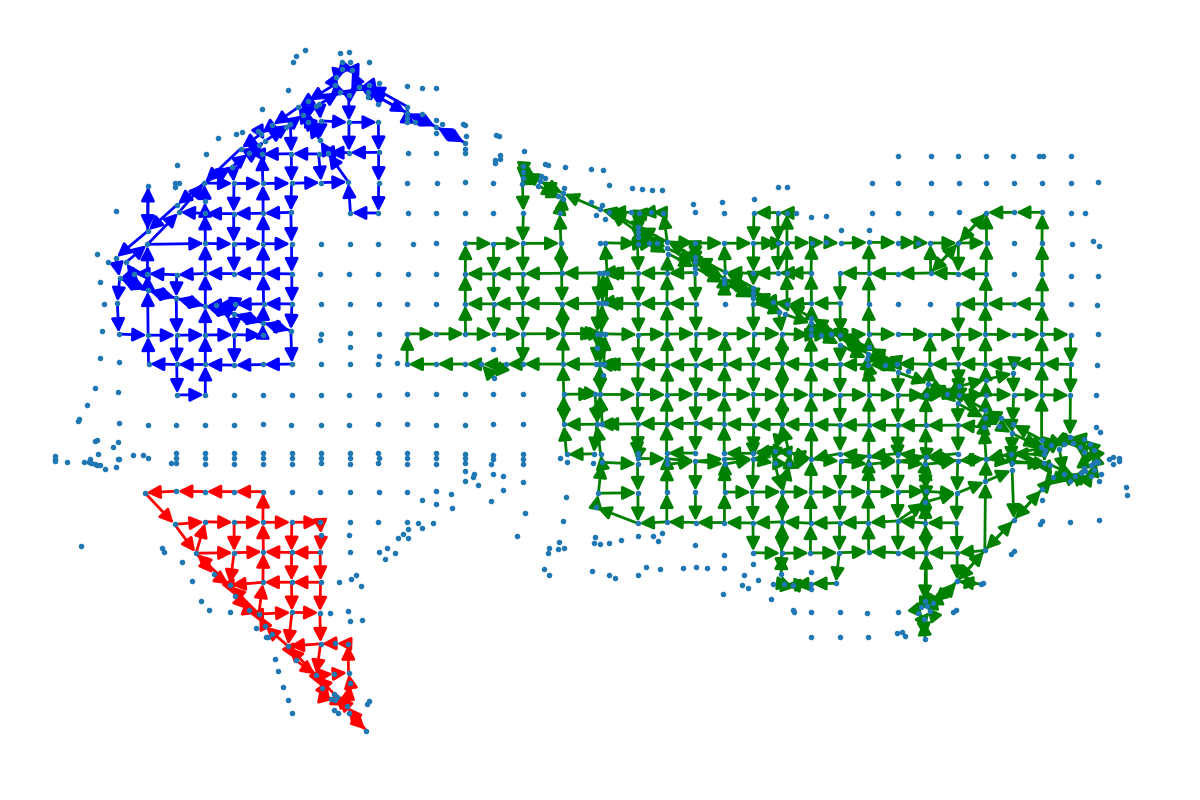
\includegraphics[width=\linewidth]{images/009.png}
    \caption{$q=0.09$}
    \label{fig: q=0.09}
\end{subfigure}
\hfill
\begin{subfigure}[b]{0.25\textwidth}
    \centering
    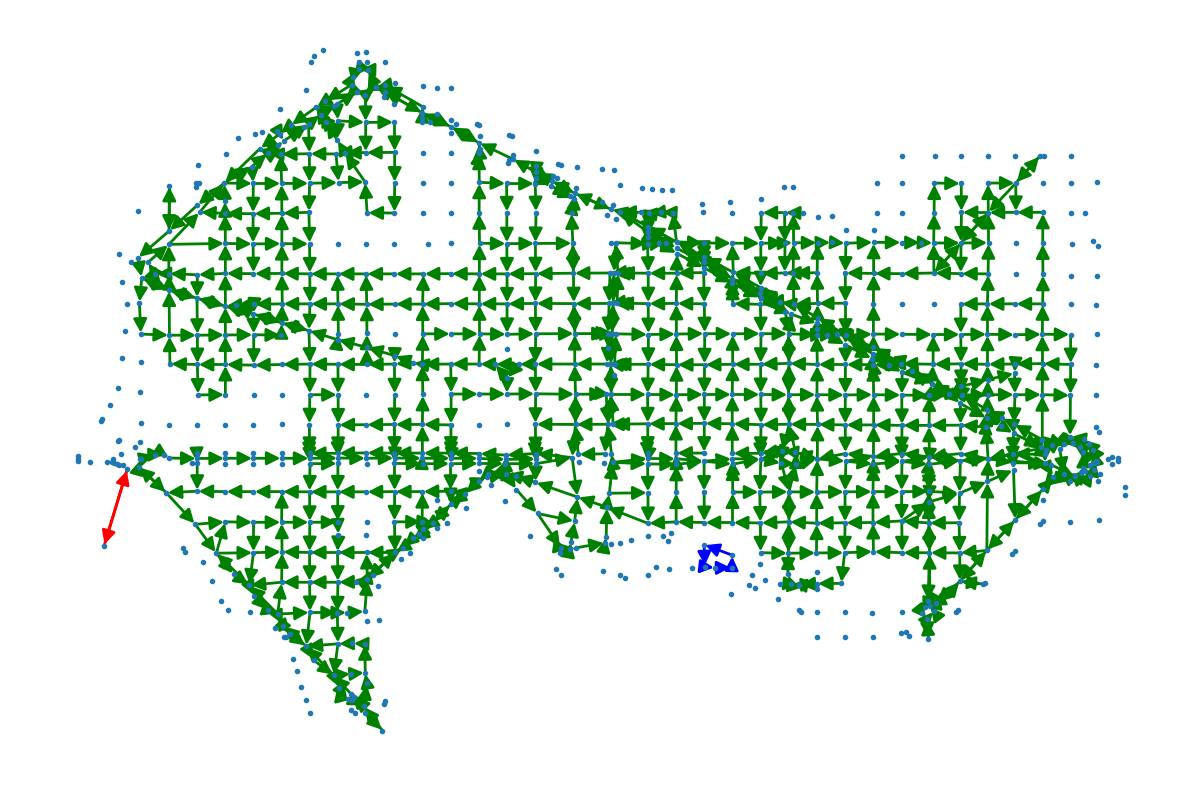
\includegraphics[width=\linewidth]{images/007.png}
    \caption{$q=0.07$}
    \label{fig: q=0.07}
\end{subfigure}
\caption{Non-congested connections with different $q$ values.}
\label{fig: conn q}
\end{figure*}

\subsubsection{Analysis of critical threshold $q_c$}
Based on the network constructing method illustrated in the previous part, a functional traffic network which related to the choice of $p$ is built. To understand the relationship between $q$ and the efficiency of the road network. We may modify the value of $q$ and investigate the construction process of the dynamical traffic network to observe the emergence of global city traffic in the network scale at a particular moment. We choose a moment that road network is congested first, and choose 3 different $q$ value. At first, for $q=0.69$, which is shown in Fig. \ref{fig: q=0.69}, only small clusters of connected high-speed roadways show up, which is unable to support global network traffic. As the value of q decreases to 0.07 in Fig. \ref{fig: q=0.07}, these small clusters combine together and a giant cluster appears, where the functional network (with lower velocity) extends to almost the full scale of original road network. According to percolation theory \cite{li2015percolation, zeng2019switch}, the size of the second-largest cluster becomes greatest at $q = 0.09$ (Fig. \ref{fig: q=0.09}), indicating the phase transition point for network connection of a functioning traffic network. To understand the percolation-like process better, the relationship between $q$ and the size of largest and second largest component is draw in Figure \ref{fig: g sg}, which depicts this percolation-like mechanism in greater detail. The size of the giant component diminishes as $q$ grows, and the second-largest cluster achieves a maximum at the critical threshold ($q_c$), which separates the fragmented and linked phases of the traffic network.

% \begin{figure}[htb]
% \centering
% \begin{subfigure}[b]{0.3\textwidth}
%     \centering
%     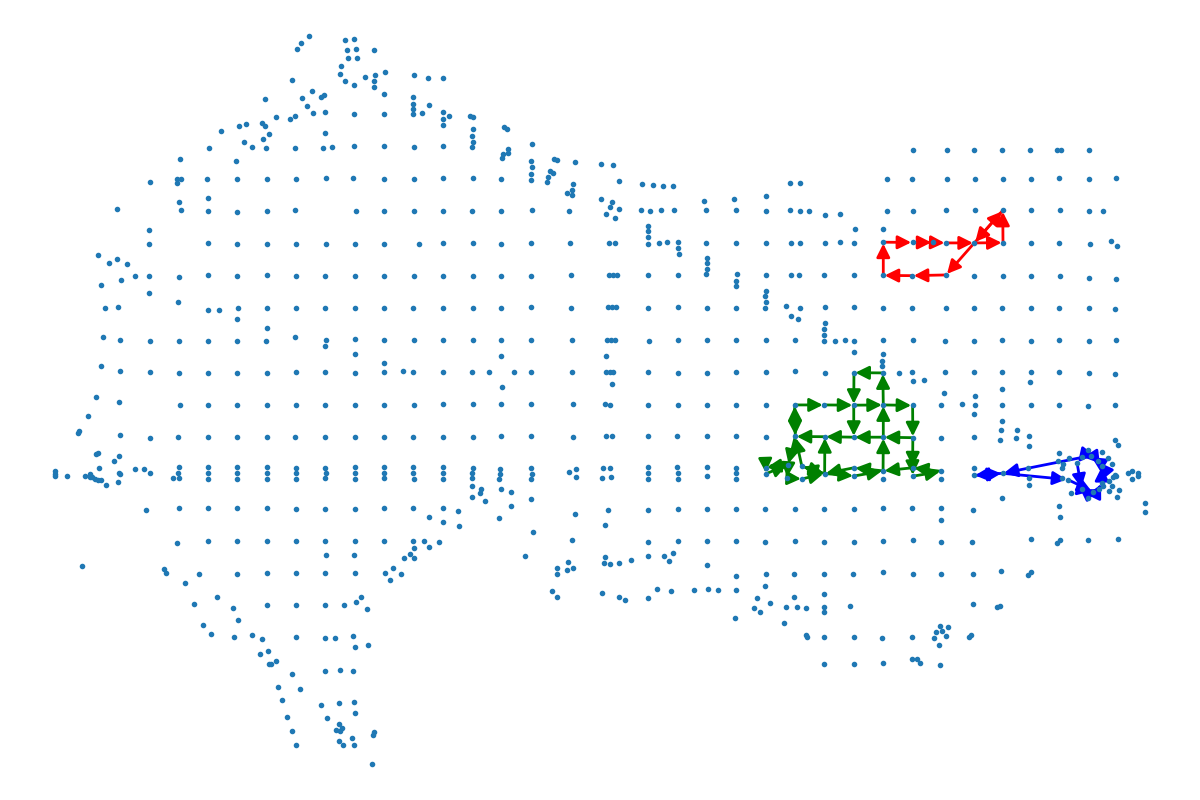
\includegraphics[width=\linewidth]{images/069.png}
%     \caption{$q=0.69$}
%     \label{fig: q=0.69}
% \end{subfigure}
% \hfill
% \begin{subfigure}[b]{0.3\textwidth}
%     \centering
%     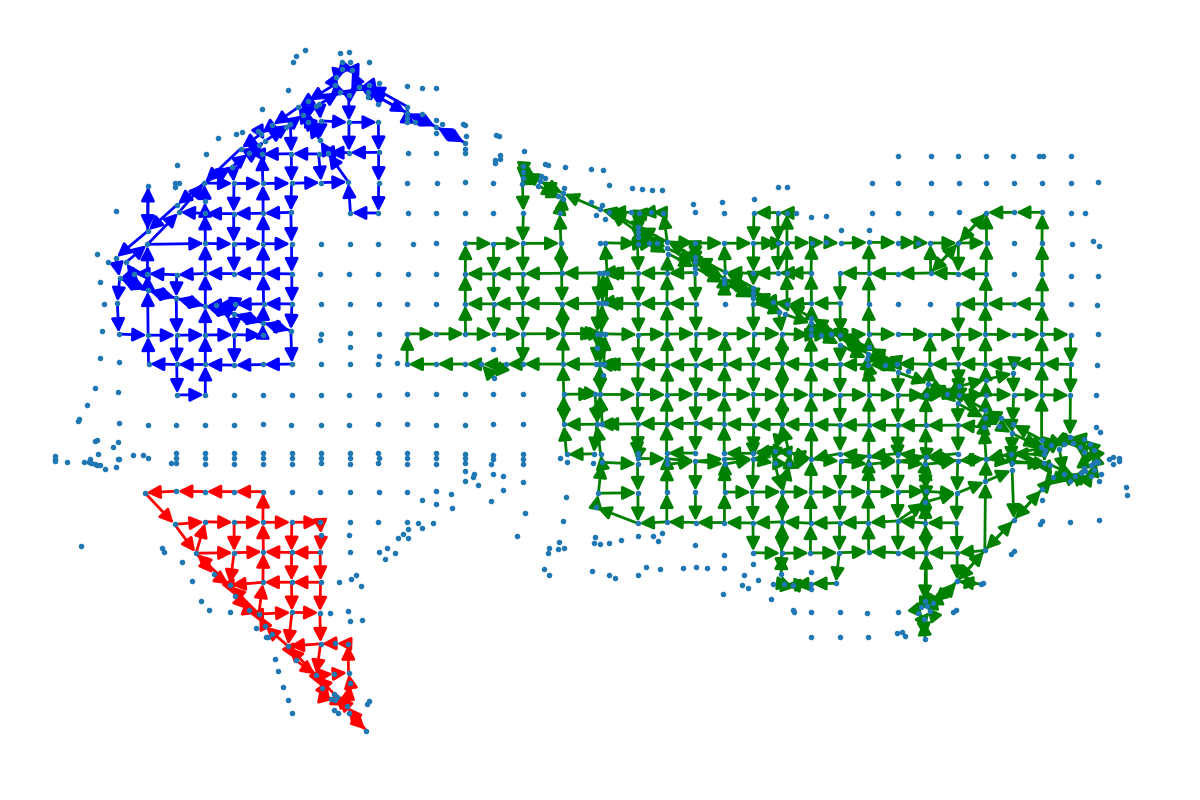
\includegraphics[width=\linewidth]{images/009.png}
%     \caption{$q=0.09$}
%     \label{fig: q=0.09}
% \end{subfigure}
% \hfill
% \begin{subfigure}[b]{0.3\textwidth}
%     \centering
%     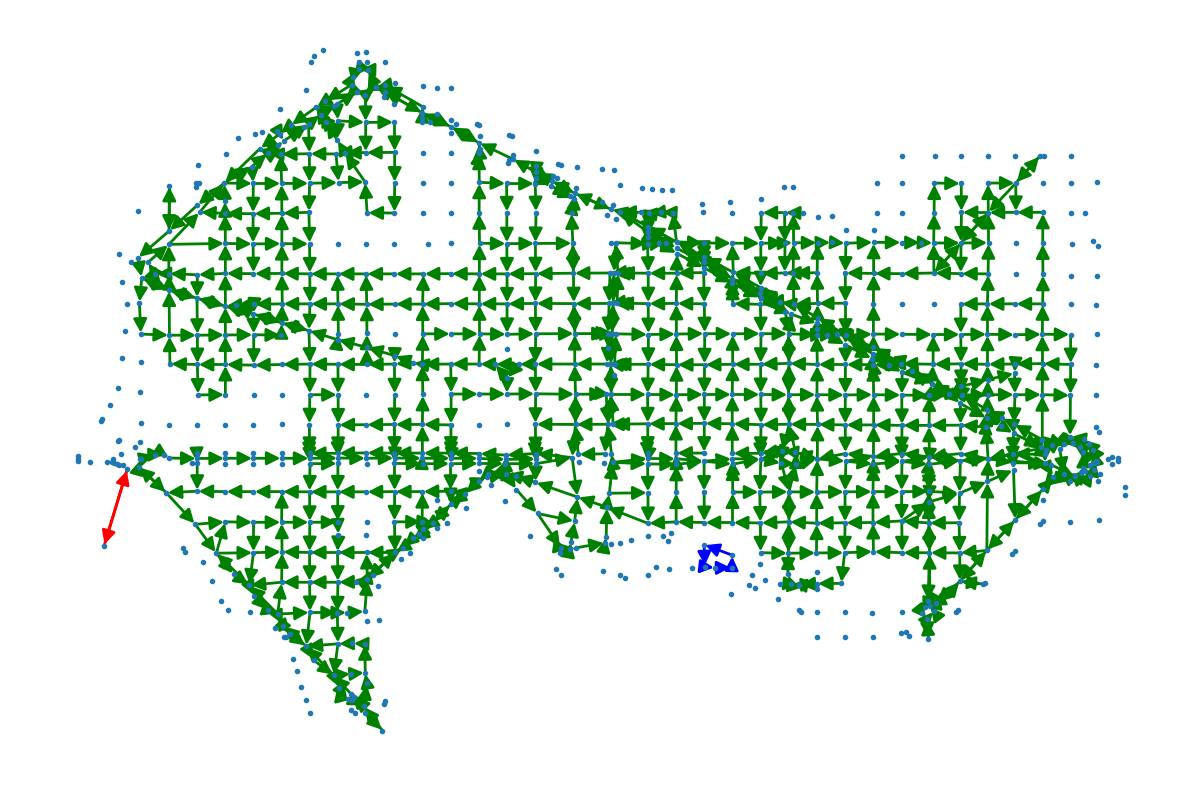
\includegraphics[width=\linewidth]{images/007.png}
%     \caption{$q=0.07$}
%     \label{fig: q=0.07}
% \end{subfigure}
% \caption{Non-congested connections with different $q$ values.}
% \label{fig: conn q}
% \end{figure}

The critical threshold $q_c$ in this percolation-like process measures the organization efficiency of real traffic as an indication of the resilience features of network connection. An individual vehicle with a speed below $q_c$ may travel the majority of the city (giant component of the traffic network), but with a velocity above $q_c$, the vehicle would be restricted in small isolated clusters. As a result, $q_c$ shows the global efficiency of traffic in a network perspective by measuring the maximum relative velocity one may travel over the major section of the network.

The traffic development causes $q_c$ to shift substantially during the target hour as seen in Fig \ref{fig: qc-t}. At the beginning of this hour, there are not so much vehicles in the whole traffic network, the $q_c$ is large, which means the whole network can function with high speed. With the increasing of the flow in the traffic network, $q_c$ starts to drop abruptly and shows a minimum around 45 minutes. Since the congestion situation starts to dissipate after this time, the $q_c$ starts to increase during the final 15 minutes.

\begin{figure}[bht]
\centering
\begin{subfigure}[b]{0.45\linewidth}
    \centering
    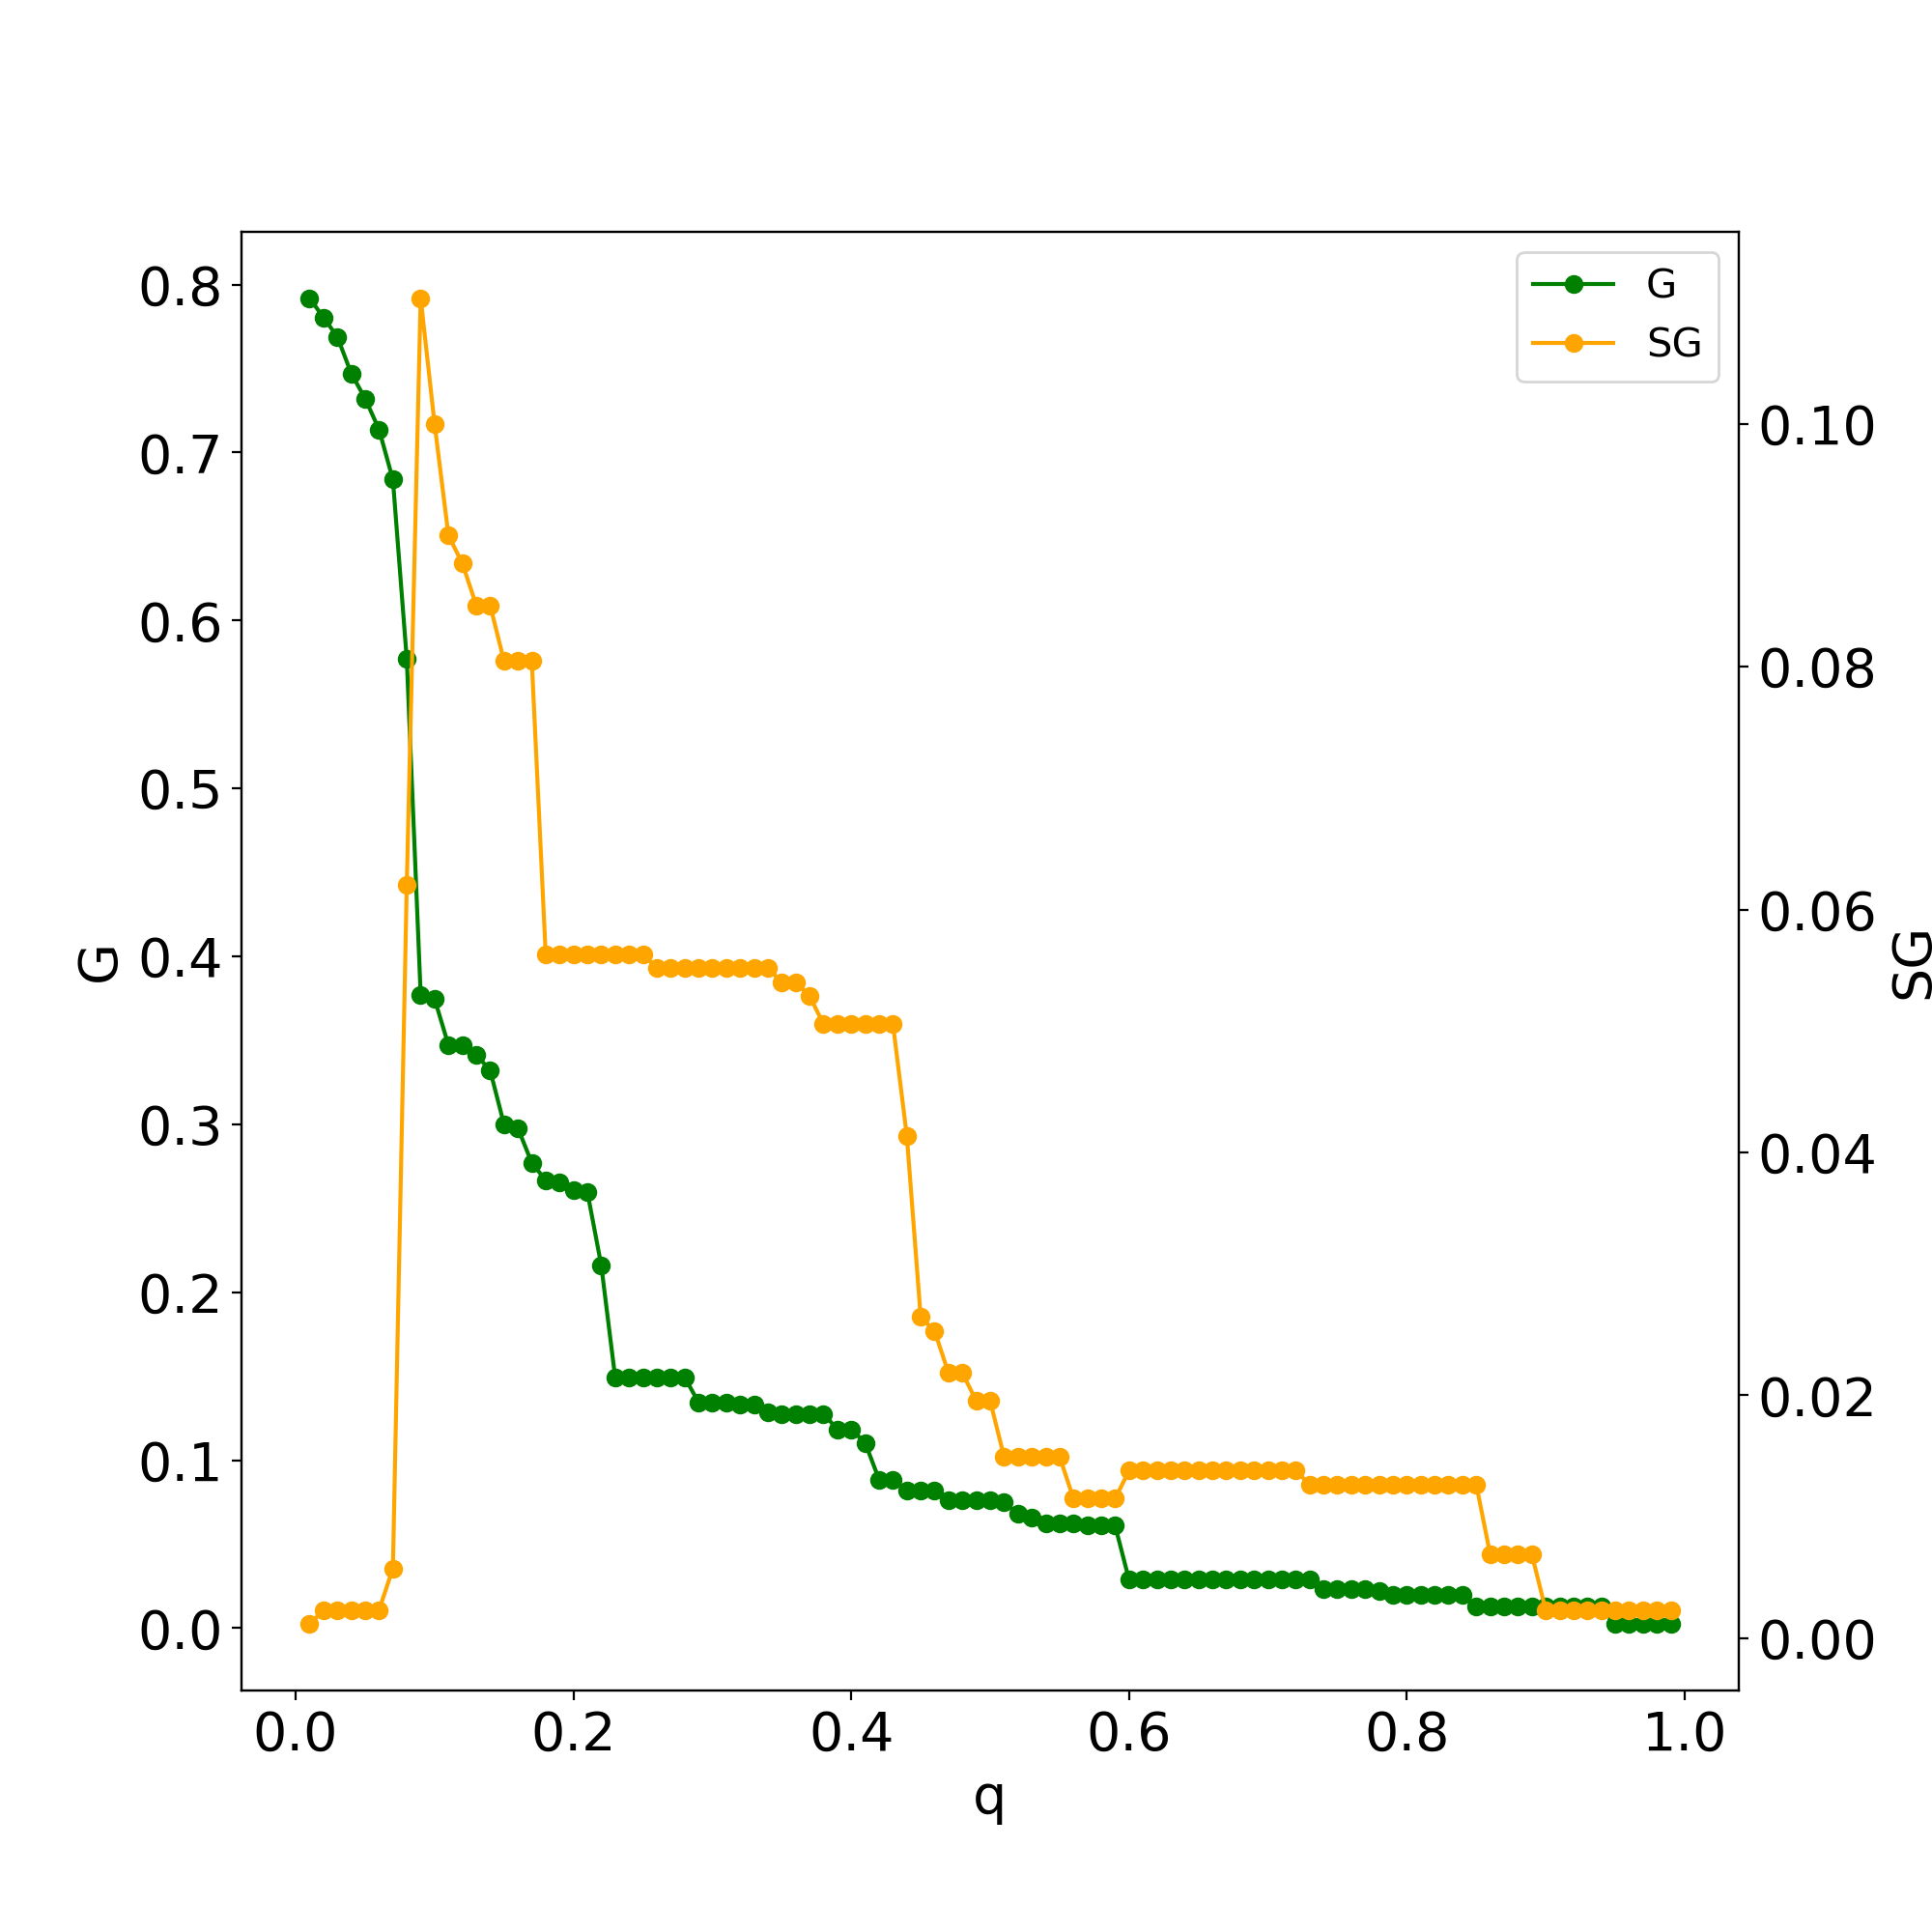
\includegraphics[width=\linewidth]{images/G and SG.png}
    \caption{}
    \label{fig: g sg}
\end{subfigure}
\hfill
\begin{subfigure}[b]{0.45\linewidth}
    \centering
    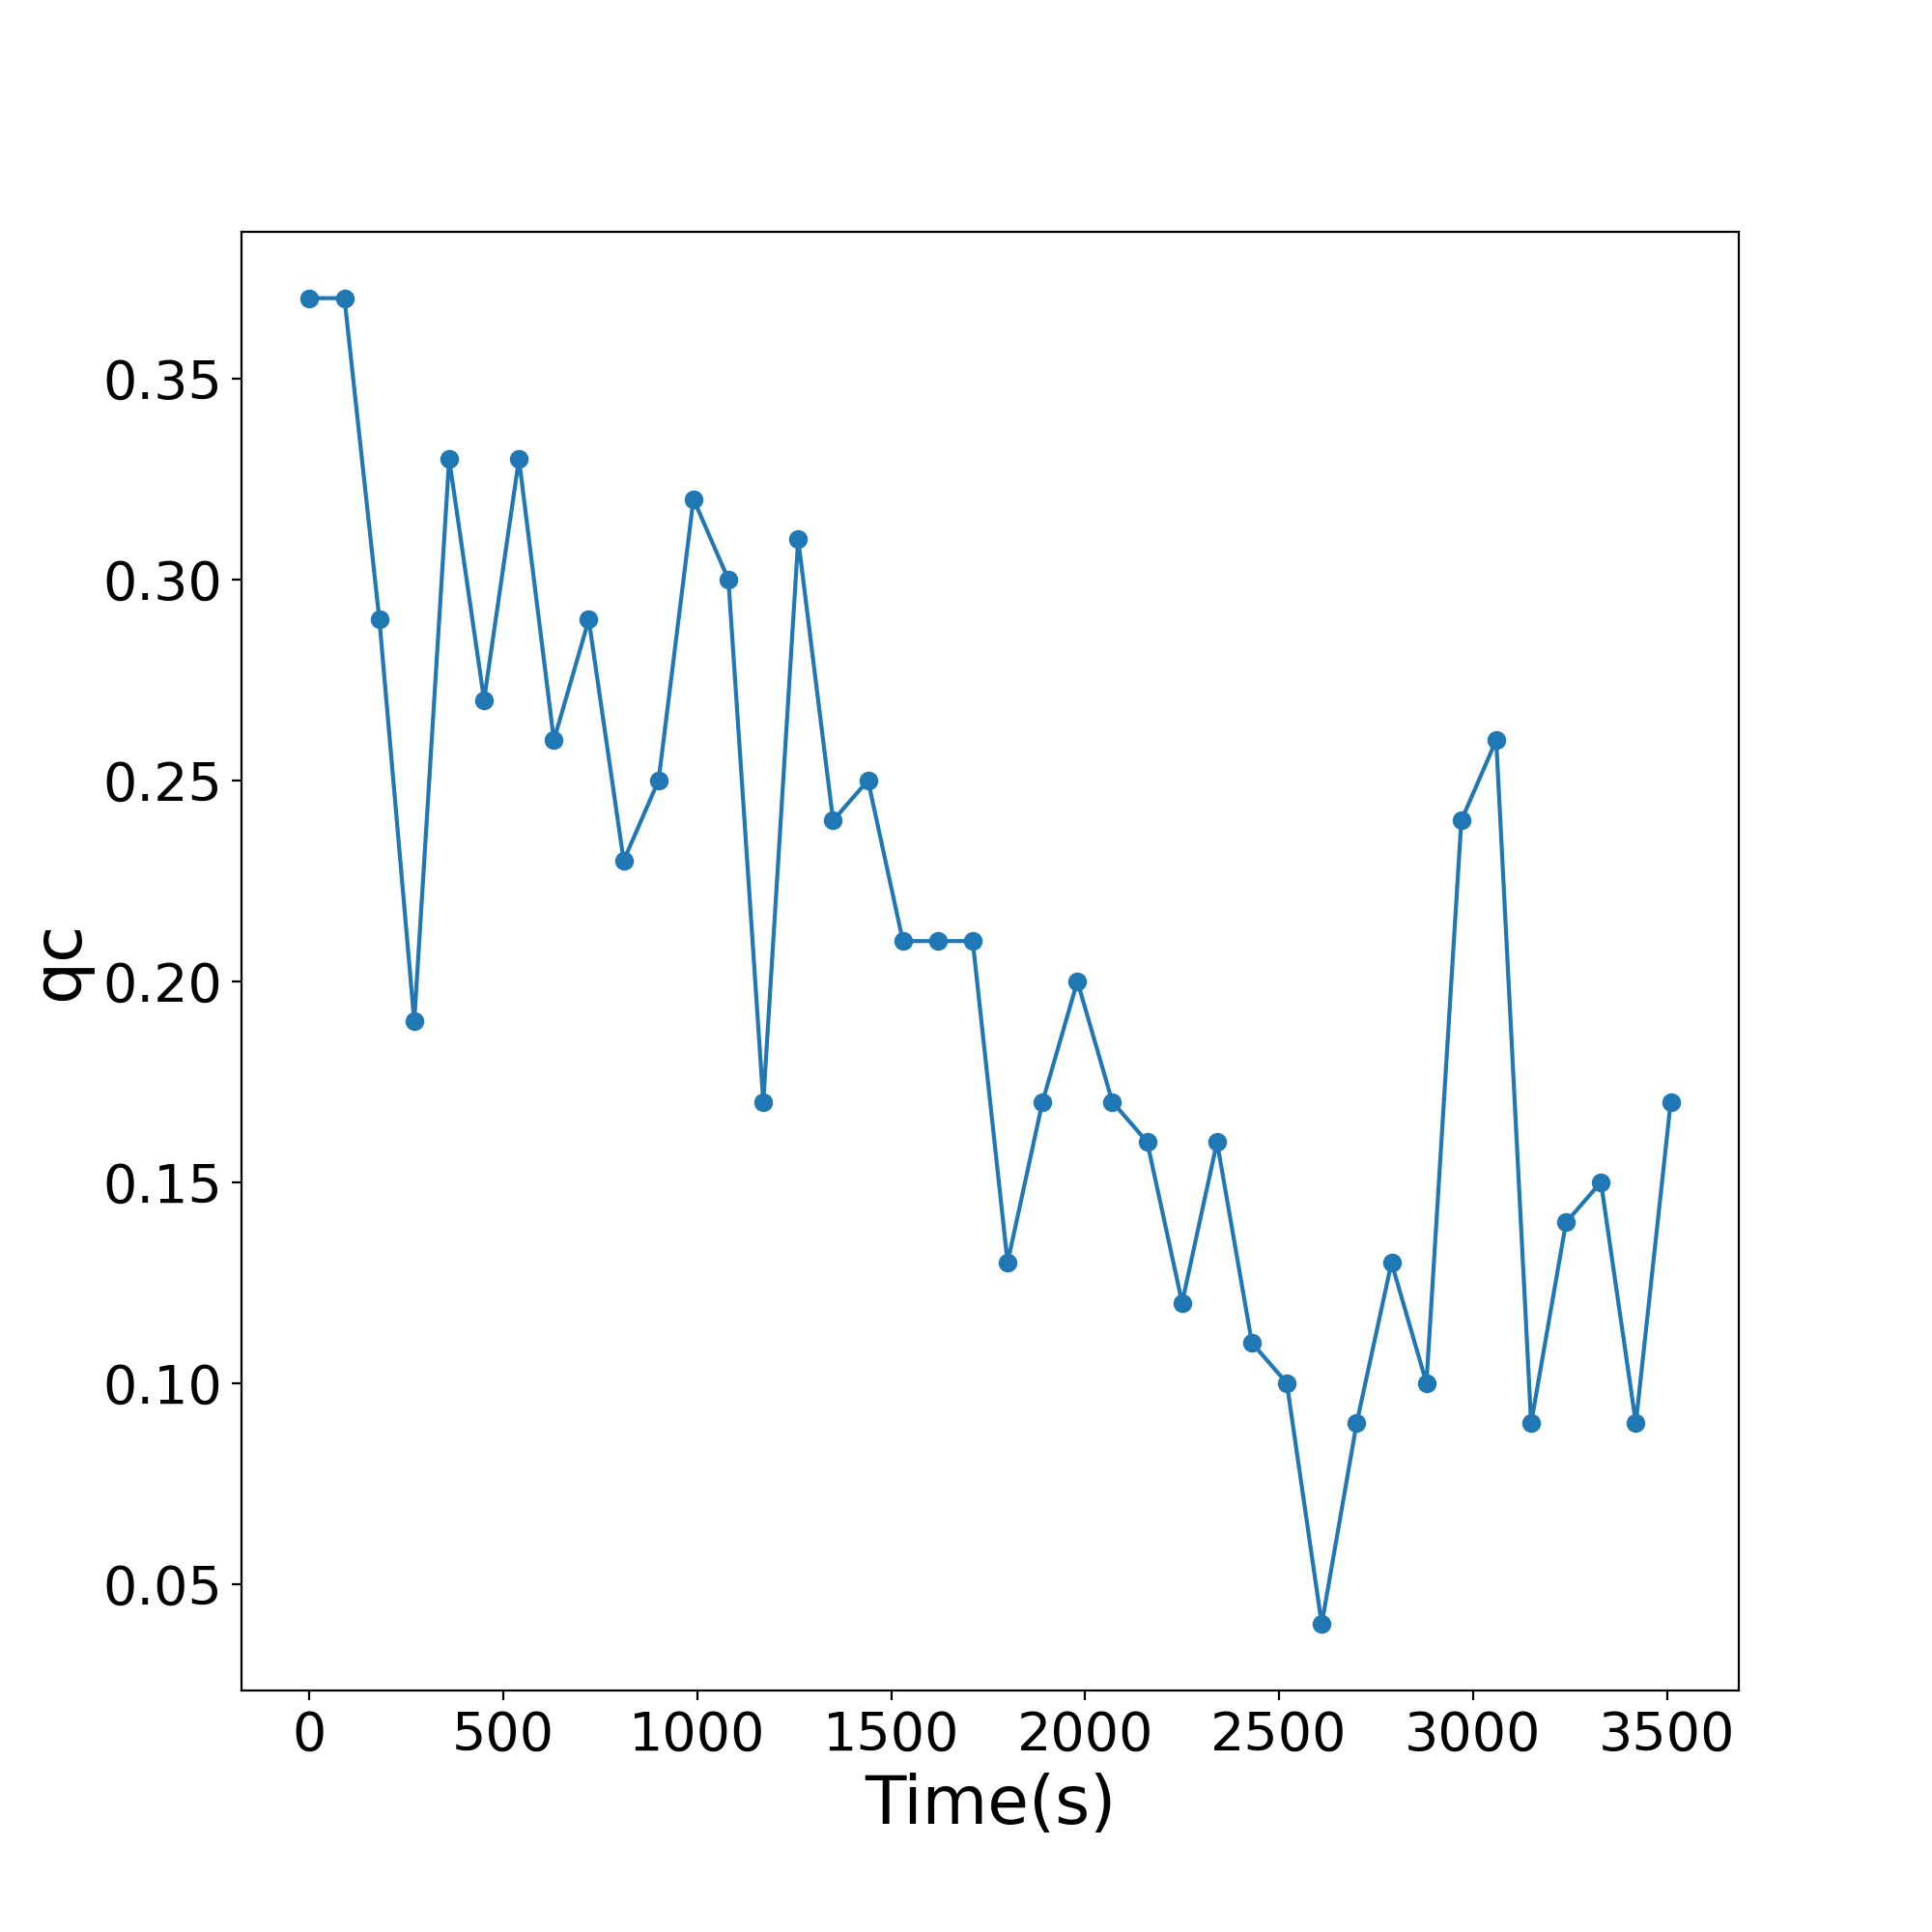
\includegraphics[width=\linewidth]{images/qc-t.png}
    \caption{}
    \label{fig: qc-t}
\end{subfigure}
\caption{(a) Relative size of the largest and 2nd largest component with $q$ value. (b) Evolution of $q_c$ w.r.t. time}
\end{figure}


\subsubsection{Critical percolation exponent}
We test the critical percolation exponent $\tau$ based on the our network construction model. As suggested in \cite{zeng2019switch}, we select $q=q_c$ as the threshold and count the connected components from the inferred graph. Let's first demonstrate one example in Fig \ref{fig: power law} to show the exponential relationship between $n_s$ and $s$. The time instance is selected arbitrary as the only purpose is to verify the correctness of (\ref{eq: power law}).

\begin{figure}[bt]
    \centering
    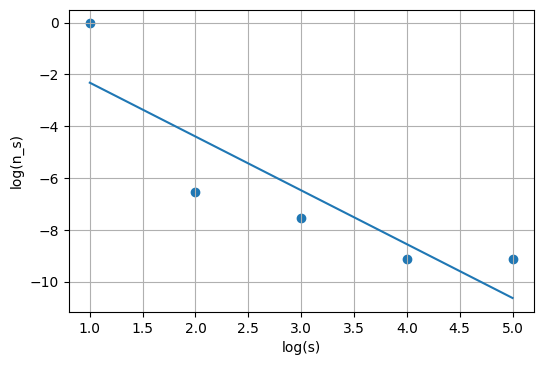
\includegraphics[width=0.7\linewidth]{images/linear_fit.png}
    \caption{Percolation cluster power law. (slope=-2.07)}
    \label{fig: power law}
\end{figure}

We calculate the evolution of $\tau$ as time progresses. The result is shown in Fig \ref{fig: tau plots}. Although the $\tau$ value should range between 2.05 and 2.5 by the percolation theory, we can surely observe that a lot of the data points are deviated from the theoretical values. We believe it's mainly because our network size is not large enough, and the network is not exact grid-like. Notice the theoretical results are derived with undirected graphs, while our road hierarchy involves multiple one-way paths. To verify this claim, we construct another network assuming all roads are two-way roads and give the result in Fig \ref{fig: tau undir}. We can see the value is more centered around 2.05 to 2.5 in undirected network than the directed one by comparing Fig \ref{fig: tau dir} and \ref{fig: tau undir}.

Nevertheless, we can still see the trend that with higher $\tau$ value, the connectivity of the network is better by observing its relationship with $q_c$. Namely, since $\tau$ is positively related to $q_c$, higher values indicates a more resilient network towards heavy traffic. One can also observe a better connectivity by the fact that the $\tau$ value is also larger in the undirected setting than its counterpart in the directed setting in general.

\begin{figure}
\centering
\begin{subfigure}[b]{0.7\linewidth}
    \centering
    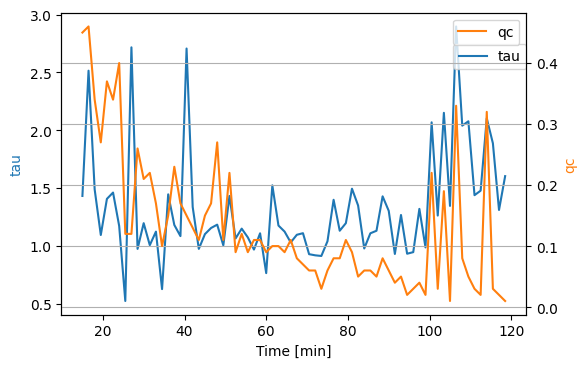
\includegraphics[width=\linewidth]{images/tau_qc_base2.png}
    \caption{$\tau(t)$ with directed network}
    \label{fig: tau dir}
\end{subfigure}
\begin{subfigure}[b]{0.7\linewidth}
    \centering
    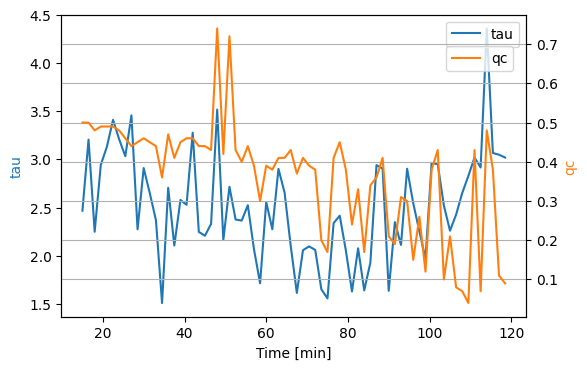
\includegraphics[width=\linewidth]{images/tau_qc_undir_base2.png}
    \caption{$\tau(t)$ with undirected network}
    \label{fig: tau undir}
\end{subfigure}
\caption{Critical percolation exponents.}
\label{fig: tau plots}
\end{figure}


\subsubsection{Bottleneck searching and discussing}
Based on the study from the research\cite{li2015percolation}, the network at percolation criticality acts as the original network's "backbone." There are some links that have a significant effect for bridging different functional clusters of traffic. Therefore, these specific links can be considered as bottlenecks, whose speed are the lowest among the links in the backbone. Fig. \ref{fig: bottleneck} illustrates the links removed at criticality. Different color represents different cluster in the graph, the orange link represents the bottleneck we find. Since road network is a directed graph, we define the component as strongly connected component, in which all pairs of nodes are mutually accessible from each other along a directed path. Therefore, if the bottleneck is removed, the giant component will disintegrate into different clusters.
\begin{figure}
\centering
\begin{subfigure}[b]{0.8\linewidth}
    \centering
    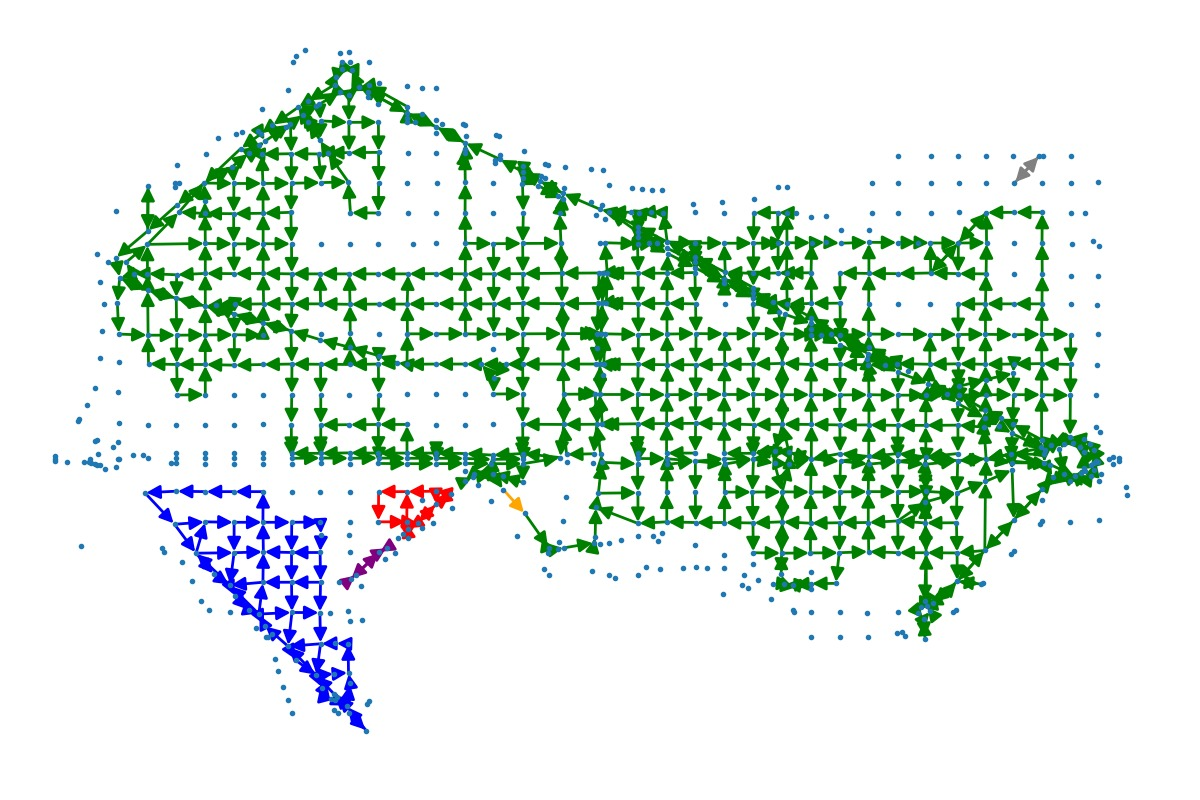
\includegraphics[width=\linewidth]{images/after.png}
    \caption{5 largest components distribution before remove the bottleneck}
    \label{fig: bottleneck after}
\end{subfigure}
\begin{subfigure}[b]{0.8\linewidth}
    \centering
    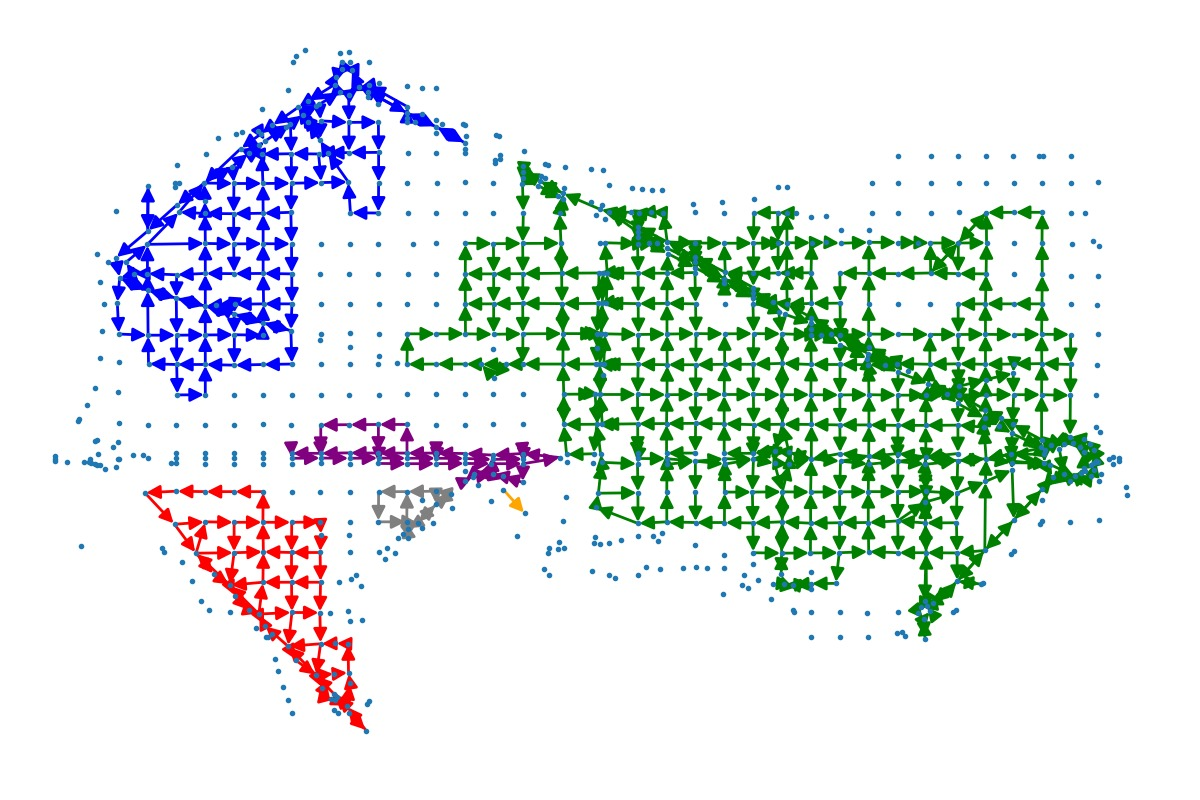
\includegraphics[width=\linewidth]{images/before.png}
    \caption{5 largest components distribution after remove the bottleneck}
    \label{fig: bottleneck before}
\end{subfigure}
\caption{the impact of bottleneck to the whole road network, the $q_c$ in (a) is 0.1, the $q_c$ in (b) is 0.09}
\label{fig: bottleneck}
\end{figure}
Besides, the bottleneck link could also have a impact for the global traffic, if the speed of bottleneck is increased, $r_{i j}^{'}=r_{i j}(1+\alpha)$, then $q_c$ of the traffic network is significantly increased. However, if we increase the link speed randomly, there is no such effect for the global network.

\section{Conclusion}
We have demonstrated a series of tools for traffic network analysis. The metrics presented in the previous sections indicate different characteristics of a traffic network. The critical threshold $q_c$ indicates the robustness of a network; the critical percolation exponent $\tau$ roughly captures the type of a network, and the connectivity of distant points.

Meanwhile, based on the finding of the impact of bottleneck, we have a deeper understanding for congestion formation and dissipation mechanisms. In the future, the control of bottleneck traffic can have a significant effect for mitigating the city traffic congestion.

\section*{Acknowledge}
The author thanks the supervisors Yura Tak and Robert Fonod for the detailed instructions during this semester, as well as the kind support from our prof. Nikolas Geroliminis.

\bibliographystyle{IEEEtran}

\bibliography{ref}

\end{document}


